The objective of this experiment is to use limiting belt friction equation given in the laboratory script to find the coefficient of friction $\mu$ of two types of belt-pulley configuration; coil friction belt configuration and vee belt configuration. The configuration used for both belt experiments is shown in the schematic below: \\
\begin{figure}[H]
\centering
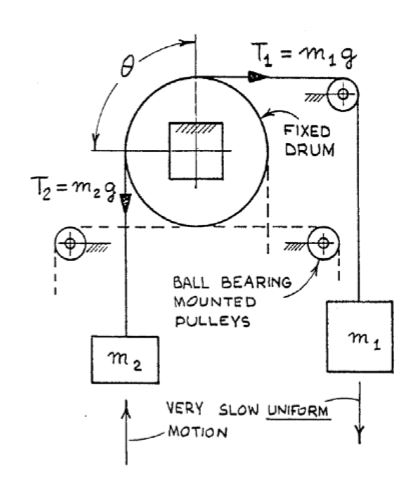
\includegraphics[width=0.5\textwidth]{chapters/lab2/setup}
\caption{Belt configuration.}
\label{fig:mesh1}
\end{figure}
Where $m_2$ is the slack tension side, $m_1$ is the tight tension side and $\theta$ is the angle of lap. Angle of lap is defined as the angle it makes between the slack tension side and the tight tension side. The configuration for the lap angle is shown on the figure below:
\begin{figure}[h!]
\centering
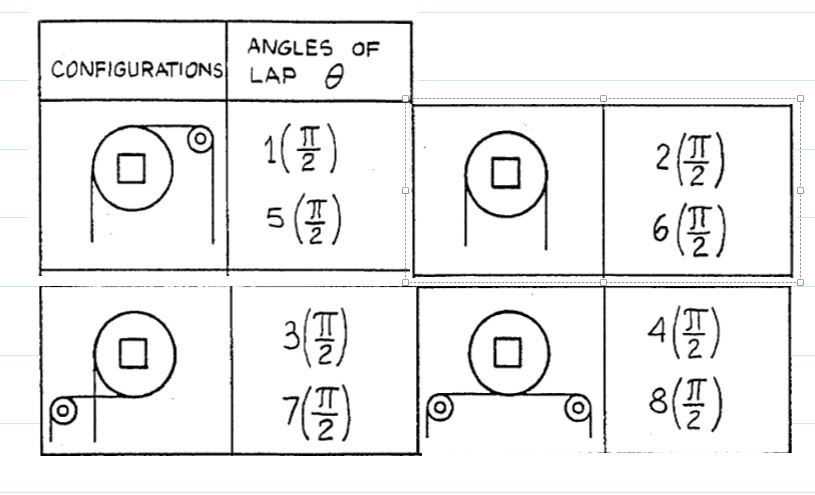
\includegraphics[width=0.7\textwidth]{chapters/lab2/angle}
\caption{Belt lap angle configuration.}
\label{fig:mesh2}
\end{figure}

The limiting belt friction relationship equation is given by:
\begin{equation}
\frac{T_1}{T_2} = e^{\mu'\theta}
\end{equation}
Where $\mu'$ is defined as:
\begin{equation}
\mu' = \mu*\csc\left(\frac{\alpha}{2}\right)
\end{equation}
Where $\alpha$ is the lap angle of the belt in the general configuration.